%=============================================================================
% DESIGN
% How is this problem to be approached, without reference to specific implementation details?

% ## Guidance

% Design should cover the abstract design in such a way that someone else might be able to do what you did, but with a different language or library or tool.
%=============================================================================

\documentclass[../main.tex]{subfiles}
\graphicspath{{\subfix{../images/}}}

\begin{document}

This chapter builds on the problems established in the previous chapter, and provide an overview of the final solutions for them, in terms of high-level technical and graphical design (architecture and interface respectively), along with justification for each decision.

\section[Considerations]{Considerations \& Principles}

As part of developing this project from scratch, there would be considerations to be made therefore establishing principles that all processes would follow. These would be in compliance with the requirements to help create a better output.

\subsection{Compatibility}

The application can be developed to be native, web-based or hybrid. With a native application, the size and performance would be highly optimised for the platform it is written for. However, this means that supporting multiple platforms would result in different codebases with different languages, even though the logic would be same. For example, many organisations write native apps for Android and iOS (such as the NHS COVID-19 App \cite{Covid19ExposureApp2022,NHSCOVID19AG2022}) that use Kotlin/Java and Swift/Objective-C respectively, and therefore there would either be separate teams, or require a lot of time to develop. Furthermore, it would be very difficult to keep the two consistent and free of bugs. A web-based application (commonly called "\textit{web-app}") would only run on a web browser and use HTML, CSS and JavaScript. These are highly compatible as browsers would be available on most platforms, and just need to get web resources. However, access to browser could still be inconvenient and have low performance (especially in mobile). Therefore, a hybrid application is a mixture of both that allows applications to run on a browser, and also run natively. There are technologies and frameworks such as \citetitle{XamarinOpensourceMobile} (C\#), \citetitle{ReactNative2022} (JavaScript) and \citetitle{Flutter2022} (Dart) that enable development of hybrid apps with one codebase.

\subsection{Extensibility}

Extending this project with new capabilities and features should not require a lot of work other than developing the extension itself. This would also mean that the system would need to be modular i.e. allowing other modules to attach to it and use the system if required. The modules themselves could also allow sub-modules to be added, but they would have to ensure that they are as independent as they can be, and encapsulate logic or concerns into the module itself. Using suitable architectures like REST (\ref{subsec:Representational State Transfer}) and Plug-ins (\ref{subsec:Plug-ins}) that would give an API, but also need to organise the codebase directory structure to workspaces.

\subsection{Durability}

To make sure that the system is durable in terms of usability, security and service, the solutions chosen should be future-proof. This means that all methods, utilities and architectures used must not be outdated. Using external dependency would mean that the points of usage of the dependency may introduce vulnerabilities. For example, if a bug is discovered in the dependency, then the application may have the bug as well. So dependencies would need to be on the latest or a long-term-support (LTS) version and the usage must be safeguarded.

\subsection{Reusability}

While the development has the privileged option of open-source that allows usage of existing, pre-developed packages that would be tested and used by a large community, every solution should not depend on these. Keeping a low number of dependencies would cause less problems, like durability as mentioned in section \ref{subsec:Durability} or a dependency hell. Where possible, they could rather be avoided, and use own constructed implementation, providing lot more flexibility.

\section{Software Architecture}

The approach to write code would be through object-oriented programming where everything would be considered as an object (or module). There would also be some usage of functional programming (through lambda\footnote{Also called anonymous or arrow in JavaScript.} functions and list comprehensions) to make code more concise.

The system architecture, however, acts as a blueprint providing abstraction of logic and complexity between components, and so it is important to consider the patterns that this project could use.

\subsection{Model View Controller}

The system would be required to be separated into three components - Model, View and Controller, each responsible for different aspects therefore enabling separation of concerns. It is important since the system is supposed to be extensible (as discussed in \ref{subsec:Extensibility}) with different modules and working with a database would mean isolating it from different concerns.

\begin{figure}
    \centering
    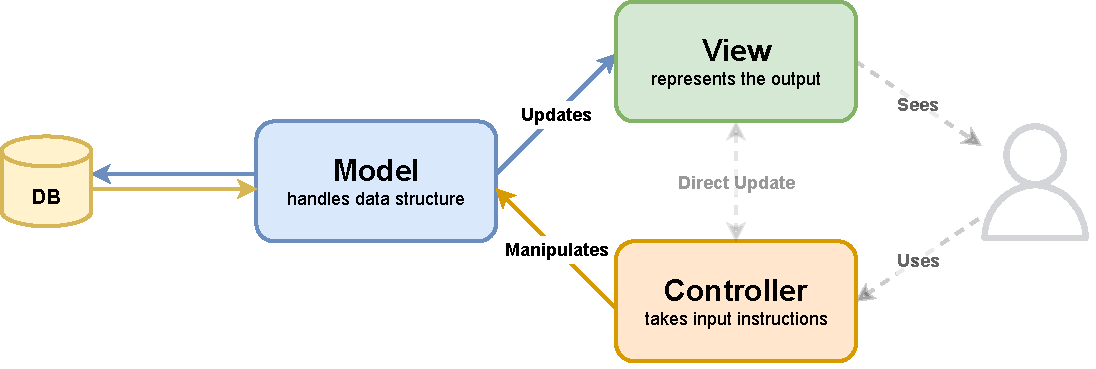
\includegraphics[width=\textwidth]{diagrams/MVC.pdf}
    \caption{Sequence diagram for Model View Controller}%\label{fig:MVC}
\end{figure}

The model, being the most important component of this pattern, requires designing the data structure which would be done with the help of a Entity Relationship diagram. This started with simple schemas of a User, "Nutrient" and their relation (figure \ref{fig:A.3}). Eventually, this was polished and finalised over development featuring important schemas (see \ref{fig:4.2}). The relationships would use the primary keys from other schemas as foreign key. For many-to-one relationships, the primary key from the single schema is used as a foreign key in the "many" side.

\begin{figure}
    \centering
    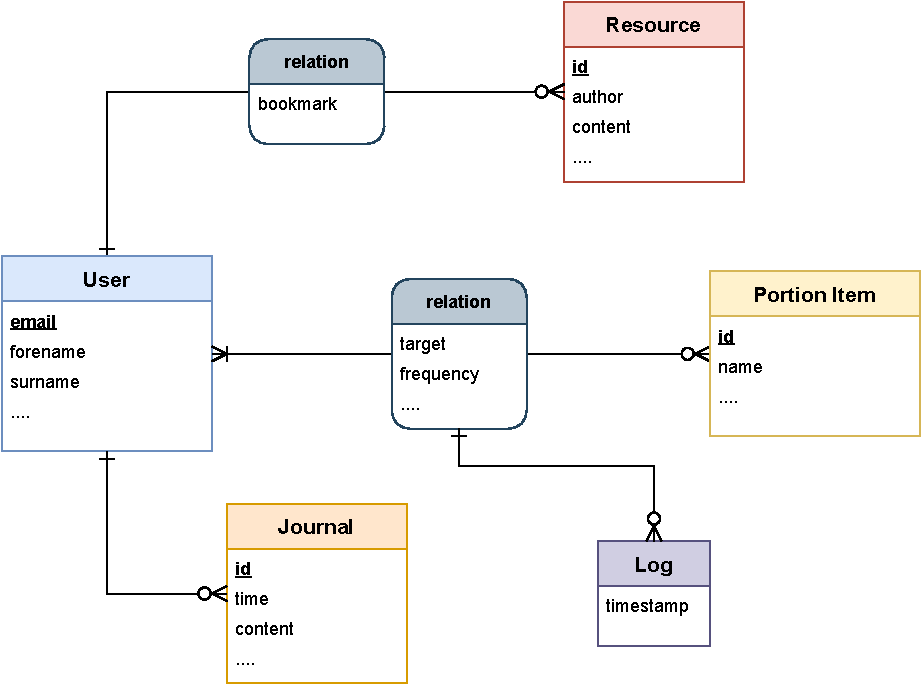
\includegraphics[width=\textwidth]{diagrams/ER.pdf}
    \caption{Entity Relationship model for the data}%\label{fig:ER}
\end{figure}

\subsection{Representational State Transfer}

It is understood that the server would be separated from client, and the client-side application could be running on multiple, different devices. The frontend interface would not deal with server logic, but would still need to exchange data at a point, like fetching previous logs or providing new ones. This would be achieved through the REST pattern (figure \ref{fig:A.4}) that allows the data to be sent and received over the World Wide Web\footnote{Using HTTP methods such as \code{GET}, \code{POST}, \code{PUT} and \code{DELETE} \cite{fieldingHypertextTransferProtocol2014}, provided users would have an internet connection.} in JSON or XML format.

\subsection{Plug-ins}

Since there is expectation with separation of concerns, extensibility and modularity, the system can be developed in a plug-in manner where each functionality would be its own plug-in that can be added or removed from the main module ("\textit{host application}").

\section{Interface Design}

The interface of the application is \textbf{critical} and \textbf{extremely important}. The user experience would majorly be determined by the design of the interface. The interface would be inspired from the paper log analysis in section \ref{sec:The Client}, and be designed in Figma \cite{FigmaPortionMate} first \cite{wikiWireframes}. This wireframe would take two iterations to get on the current stage - the first did not make use of checkboxes and had repetitive text saying "X portions taken" (see \ref{fig:A.5}). However, on further brainstorming, the right-side buttons were retained, and checkboxes were added instead to provide additional methods of input. The interface is minimal (like material design), and used dark mode by default - this was switched to light mode when the supervisor preferred it. Aside from the ones in section \ref{sec:Considerations}, there would be considerations made for the interface specifically.

\begin{figure}
    \centering
    \noindent\begin{subfigure}{.24\textwidth}
    \centering
    \frame{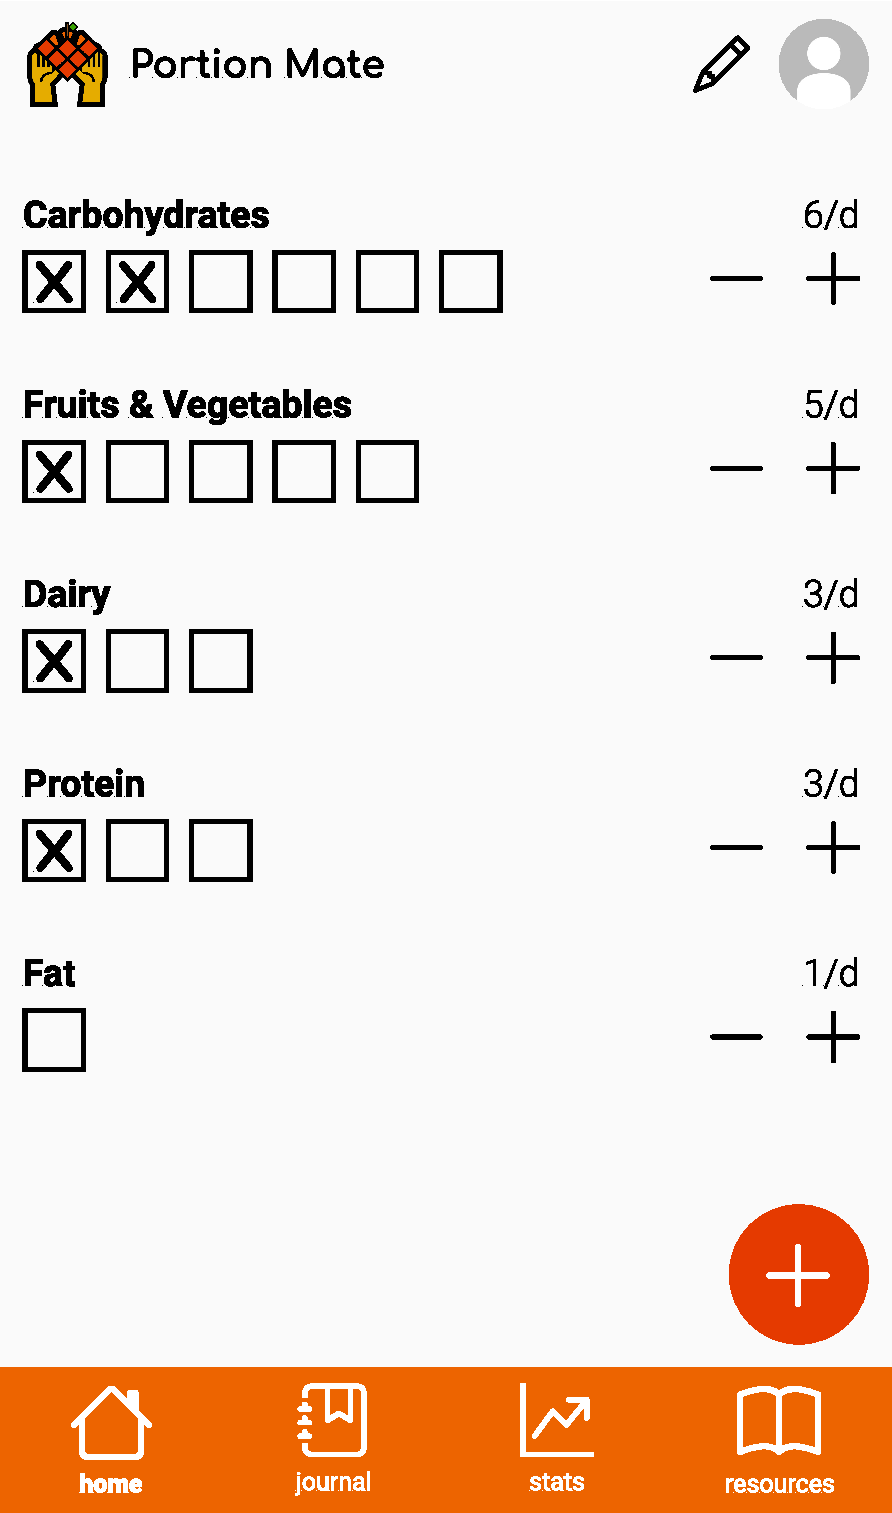
\includegraphics[height=5cm]{wireframes/Landing [home] [light].pdf}}
    \caption{Home Page}
    \end{subfigure}\hfill
    \begin{subfigure}{.24\textwidth}
    \centering
    \frame{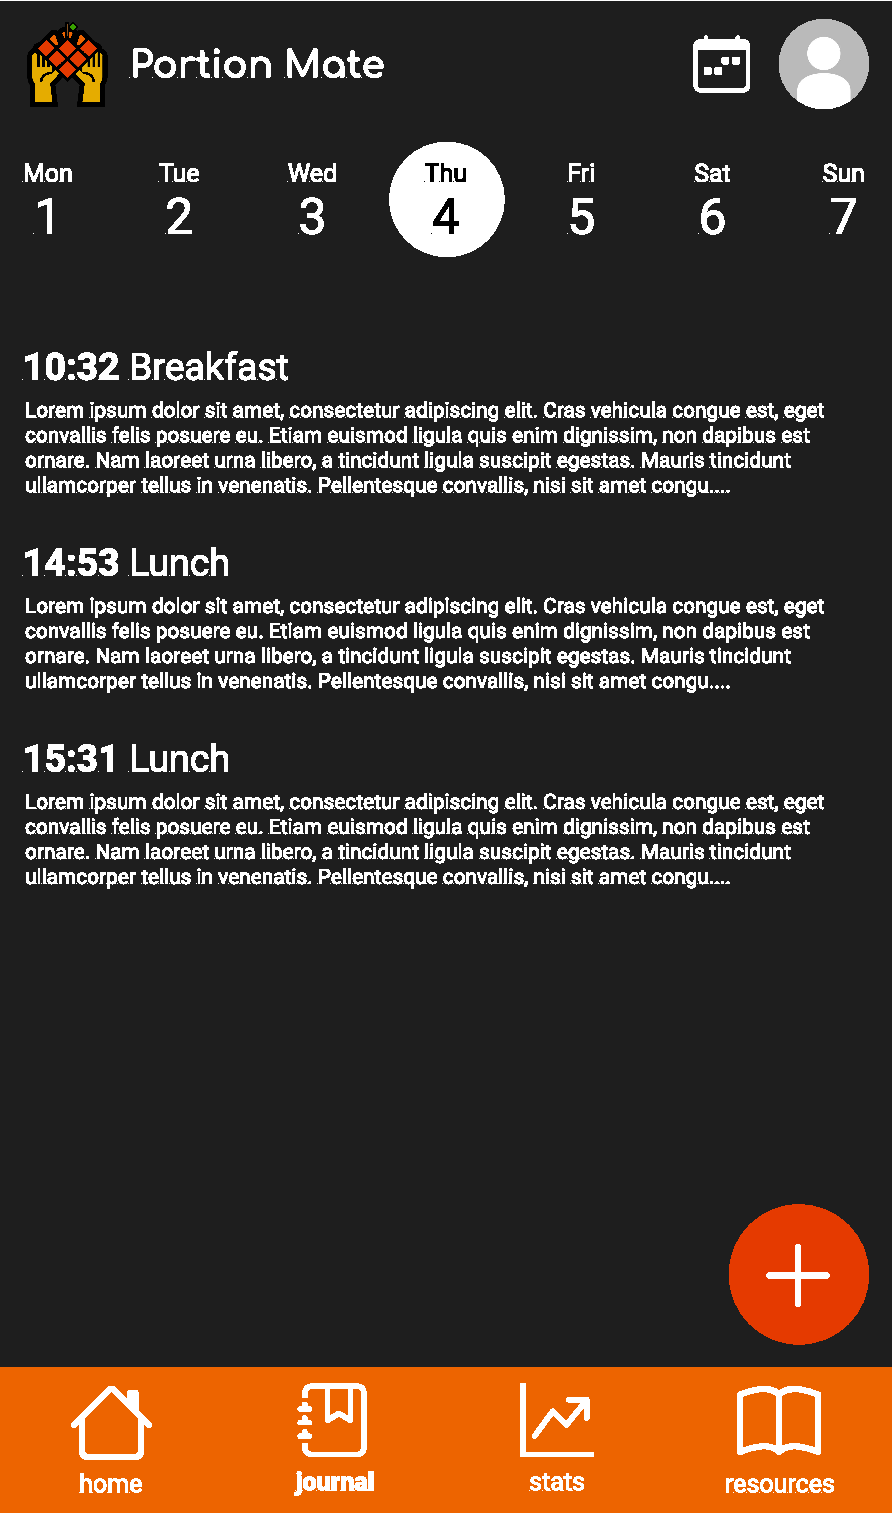
\includegraphics[height=5cm]{wireframes/Journal w Entries [dark].pdf}}
    \caption{Journal}
    \end{subfigure}\hfill
    \begin{subfigure}{.24\textwidth}
    \centering
    \frame{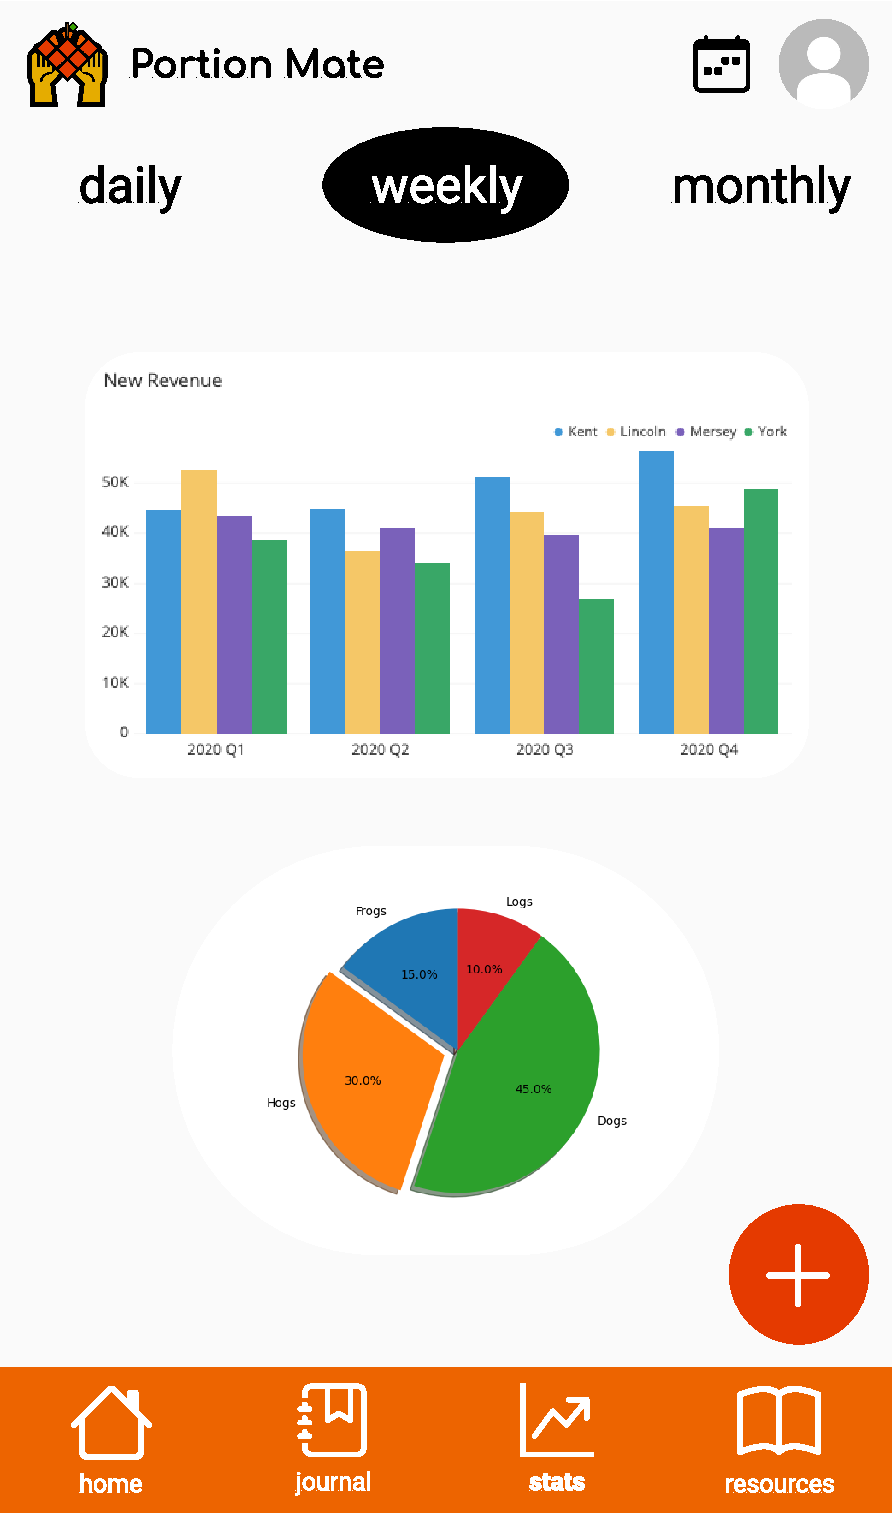
\includegraphics[height=5cm]{wireframes/Stats [light].pdf}}
    \caption{Statistics}
    \end{subfigure}\hfill
    \begin{subfigure}{.24\textwidth}
    \centering
    \frame{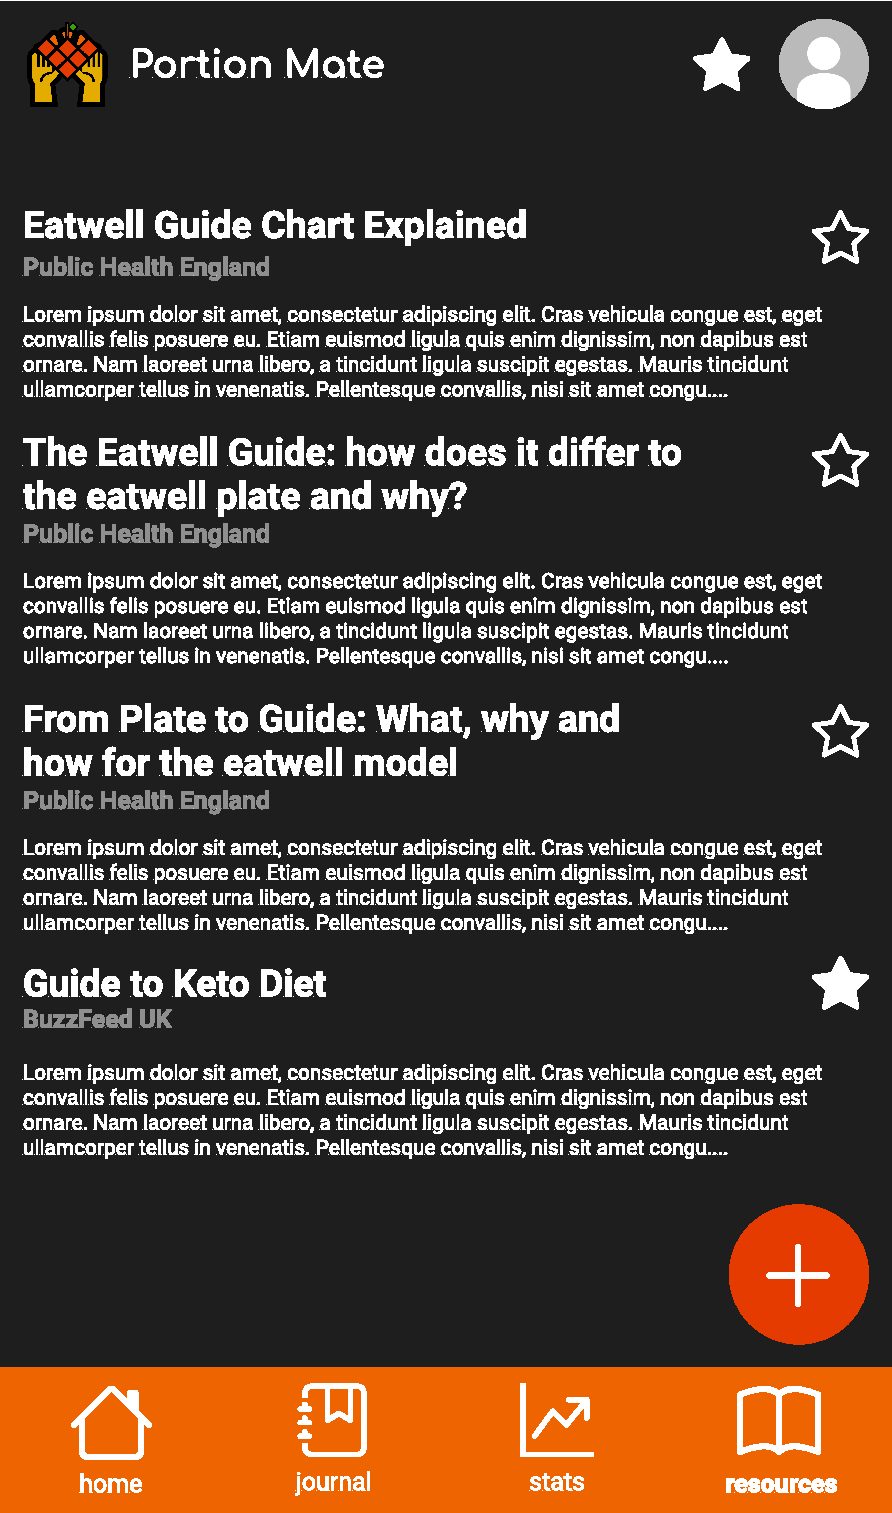
\includegraphics[height=5cm]{wireframes/Resources [dark].pdf}}
    \caption{Resources}
    \end{subfigure}
    \caption{Wireframes from \citecode{FigmaPortionMate}}%\label{fig:wireframes}
\end{figure}

\subsection{Consistency}

The design would need to be consistent throughout the application and introduce no screen that looks very different from any others, else it would frustrate users to learn and understand a new layout, violating Nielsen's Heuristic 4 \cite{experience10UsabilityHeuristics}. An app-wide colour scheme would allow the application give identity and make the screen similar. This would also include font selection, icons, and element sizing - all should be from the same family and use consistent, proportionate numbers. The interface must also be consistent for different screen sizes (responsiveness) and not change interface drastically for a specific breakpoint or platform, like WhatsApp has very different interfaces for Android and iOS\footnote{Both operating systems, however, have their own design philosophies.} (see \ref{fig:4.4}). The same goes for toggling between light and dark mode where the interface should not become unfamiliar on changing themes.

\begin{figure}
    \centering
    \noindent\begin{subfigure}{.49\textwidth}
    \centering
    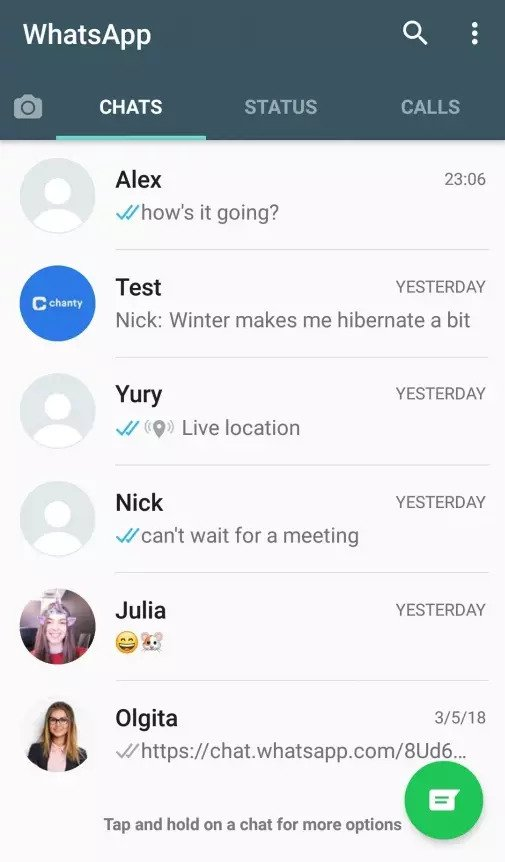
\includegraphics[height=8cm]{screenshots/whatsapp_android.jpg}
    \caption{WhatsApp on Android}
    \end{subfigure}\hfill
    \begin{subfigure}{.49\textwidth}
    \centering
    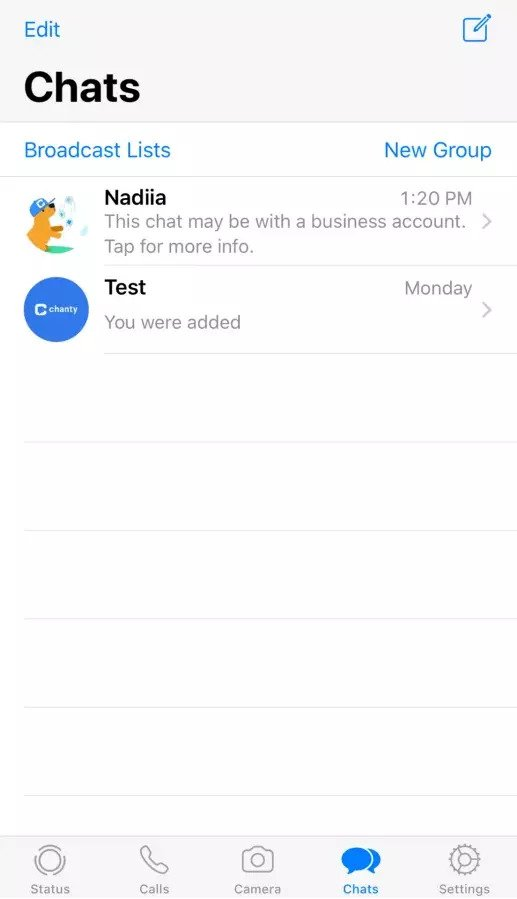
\includegraphics[height=8cm]{screenshots/whatsapp_ios.jpg}
    \caption{WhatsApp on iOS}
    \end{subfigure}
    \caption{Very different interfaces for WhatsApp (\textit{from Chanty})}%\label{fig:WhatsApp}
\end{figure}

\subsection{Accessibility}

The interface would need to be accessible, otherwise it would limit users on their actions and cause frustration. There are guidelines that instruct and define rules to make accessible interfaces, such as W3C \cite{AccessibilityW3C}. First, the basic elements need to be considerate and inclusive. The images and icons would require \code{alt} property that can be picked up by screen-readers as they read through each element and parse the HTML code. The font face should be legible and enable users to distinguish between letters; sans-serif fonts, like Arial and Verdana, are preferable. Roboto was designed and released by Google in 2011 for Android \cite{GoogleUnwrapsIce}, and has become popular for its clean and modern look. Differentiation should not depend on colours, but can also use other means of displaying hierarchy through text weight, positioning and icons. A responsive design would also enable the interface to be accessible on screens of various sizes\footnote{From 8K large displays to palm-sized 360p; watch faces would highly differ.}. As the application allows switching between light and dark mode, that can help with eye strain, but the ability to toggle should be easily available through the system (and saving the preference).

\section*{Summary}

Users and developers are human, and since the project focuses on Human Computer Interaction, the design decisions were critical. Making these decisions would lay the foundation for the application as they define principles for the development process. Any written code should be modular so that it could be extended with more functionalities if required. The policy on external dependencies asks to use recommended versions, but avoid usage wherever possible. The architectural patterns that the technology would use include definition for the database model, and interfaces to interact with each component such as the server (from the client) and the database itself. More importantly, the interface design which would be the first element visualised by all users, and providing a method of using the application - so it needs to be inclusive and considerate, meaning that the design should be visually appealing and accessible through devices of different nature, following all guidelines and expectations. This interface would be refined from the wireframes that were constructed and prototyped before the final implementation.

\end{document}
